\documentclass[a4paper,12pt]{report}

\usepackage{cmap}
\usepackage[T2A]{fontenc}
\usepackage[utf8]{inputenc}
\usepackage[russian]{babel}
\usepackage{amsmath,amsfonts,amssymb}
\usepackage{graphicx}
\usepackage{sidecap}
\usepackage{wrapfig}
\usepackage{indentfirst}

\begin{document} 

\begin{titlepage} 

\begin{center} 

\large Федеральное государственное автономное образовательное учреждение высшего образования «Санкт-Петербургский государственный электротехнический университет «ЛЭТИ» им. В.И. Ульянова (Ленина)»\\
кафедра Вычислительной техники\\[5cm] 

\huge ОТЧЕТ\\ по лабораторной работе № 2\\[0.5cm] 
\large <<Обработка одномерных массивов>>\\[3.7cm]

\begin{minipage}{1\textwidth}
    \begin{flushleft}
        \emph{Автор:} Стукен В.А.\\
        \emph{Группа:} 2307\\
        \emph{Факультет:} ФКТИ\\
        \emph{Преподаватель:} Аббас Саддам Ахмед\\
    \end{flushleft}
\end{minipage}

\vfill

Санкт-Петербург, 2022\\
{\large \LaTeX}

\end{center}
\thispagestyle{empty}
\end{titlepage}

\section*{Задание(вариант 13)}
Дан массив вещественных чисел. Определить, есть ли в нем отрицательные числа. В случае положительного ответа:
\par
а)определить номер первого из них и вывести все следующие за ним элементы;
\par
б)определить номер последнего из них и вывести все элементы, расположенные слева от него.

\section*{Постановка задачи и описание решения}
\par
Программа получает на вход размер массива и на следующей строке сами элементы массива.
Далее идем по массиву циклом for с условием, что $num=-1$ пока не встретим отрицательный элемент. Когда встречаем его, в переменную $num$, изначально равную -1 записываем индекс этого элемента.
Если после прохождения циклом массива значение переменной $num$ осталось равным -1, то возвращаем "NO", что означает, что в массиве нет отрицательных элементов, иначе возвращаем "YES" и далее приступаем к выводу элементов массива слева и справа от первого отрицательного:
проходимся циклом for до номера этого элемента и выводим все эти элементы массива, так же соотвественно делаем с конца, выводя элементы, стоящие после первого отрицательного. 

\section*{Описание переменных}
\begin{centering}
\resizebox{14cm}{!}{
    \begin{tabular}{|l|l|l|l|}
        \hline
        \textbf{№} & \textbf{Имя переменной} & \textbf{Тип} & \textbf{Назначение}\\
        \hline
        1 &   mas          &double& Массив вещественных чисел\\ 
        \hline
        2 &   n            & int  & Размер массива\\ 
        \hline
        3 &  num           &  int & Номер первого отрицательного числа \\ 
        \hline
    \end{tabular}
}
\end{centering}

\section*{Контрольные примеры}

\begin{centering}
\resizebox{14cm}{!}{
    \begin{tabular}{|l|l|}
        \hline
          \textbf{Входные данные} & \textbf{Выходные данные}\\
        \hline
        5;      
        1 2 3 4 5                 &  NO  \\ 
        \hline
        7;
        1 4 6 -8 4 6 7            &  YES; 146; 467    \\ 
        \hline
        10; 0 4 6 7 89 45 12 -10000 78 45 2 5 & YES; 0 4 6 7 89 45 12; 78 45 2 5  \\ 
        \hline
    \end{tabular}
}
\end{centering}
\newpage

\section*{Примеры использования программы}
    \begin{figure}[h]
        \includegraphics[width=0.8\textwidth]{ex11.jpg}
    \caption{Входные данные 1}
    \label{ris:image}
            
        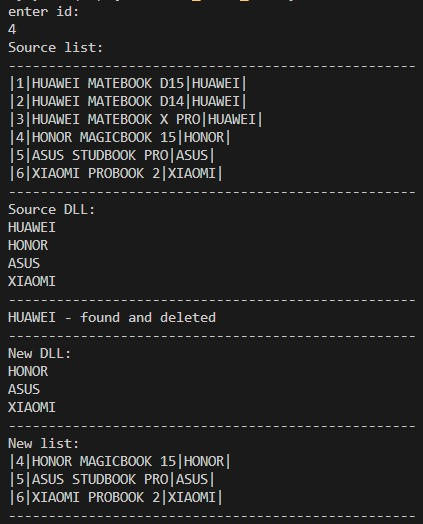
\includegraphics[width=0.8\textwidth]{ex2.jpg}
    \caption{Входные данные 2}
    \label{ris:image}
    
        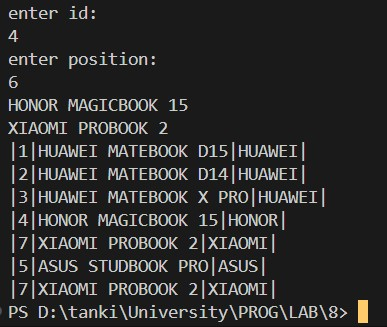
\includegraphics[width=0.8\textwidth]{ex3.jpg}
    \caption{Входные данные 3}
    \label{ris:image}
\end{figure}

\section*{Вывод}
В результате выполнения лабораторной работы изучили работу с одномерными массивами в языке Си, научились обрабатывать их элементы.

\end{document}